\documentclass[tikz, crop, border = {2pt 2pt 2pt 2pt}]{standalone}

\usetikzlibrary{patterns}
\usetikzlibrary{decorations.pathreplacing}
\usepackage{siunitx}
\usepackage{physics}
\AtBeginDocument{\RenewCommandCopy\qty\SI}
\usepackage{concmath-otf}

\begin{document}
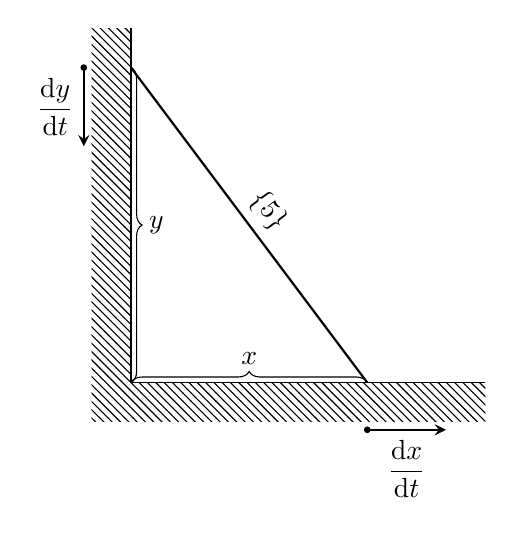
\begin{tikzpicture}
    \fill[pattern = north west lines] (0, 0) -- (4.5, 0) -- (4.5, -0.5) -- (-0.5, -0.5) -- (-0.5, 4.5) -- (0, 4.5) -- cycle;
    \draw (0, 4.5) |- (4.5, 0);
    \draw[thick] (3, 0) -- (0, 4) node[midway, auto, sloped]{$\qty{5}{\meter}$};

    \coordinate (a1) at (3, -0.6);
    \draw[thick, -stealth] (a1) -- ++ (1, 0) node[midway, auto, swap]{$\displaystyle\dv{x}{t}$};
    \filldraw (a1) circle (1pt);

    \coordinate (a2) at (-0.6, 4);
    \draw[thick, -stealth] (a2) -- ++ (0, -1) node[midway, auto, swap]{$\displaystyle\dv{y}{t}$};
    \filldraw (a2) circle (1pt);

    \draw[decorate, decoration = {brace, mirror, amplitude = 4pt}] (0, 0) -- (0, 4) node[midway, right = 3pt]{$y$};
    \draw[decorate, decoration = {brace, amplitude = 4pt}] (0, 0) -- (3, 0) node[midway, above = 3pt]{$x$};
\end{tikzpicture}
\end{document}